\section{Installazione ed avvio di SSD}
Per installare ed avviare l'applicativo "SSD" bisogna i seguenti passaggi.
\subsection{Come scaricare il programma e le librerie}

\begin{itemize}
	\item \textbf{Scaricare}: tutto il programma è presente nella seguente Repository:\newline{}
\centerline{\url{https://github.com/MercurySeven/project-SSD}}

	\item \textbf{Estrarre il contenuto del file .zip}: In una cartella a piacimento che sia al di fuori della cartella che si vuole sincronizzare utilizzare l'applicativo del computer utilizzato (7zip, Winrar, etc) per estrarre l'archivio nella cartella desiderata;
	\item \textbf{Installare le librerie richieste}:
	Arrivando tramite il terminale alla cartella dove si è estratto il contenuto dell'archivio eseguire il seguente comando:\newline{}
	\centerline{\texttt{pip install -r "requirements.txt"}}
\end{itemize}
\subsection{Come impostare PYTHONPATH}
Per impostare il PYTHONPATH bisogna utilizzare la keyword set su windows e la keyword export su macOS e Linux. La variabile deve essere impostata al path assoluto dove si è estratto l'archivio.
Di seguito sono riportati due esempi, rispettivamente per windows e linux/macOS
\begin{figure}[H]
    \centering
    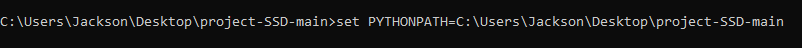
\includegraphics[scale = 0.65]{components/img/Windows-istruzione-1.png}
    \caption{Comando per impostare PYTHONPATH su windows}
    \label{fig:comando per impostare PYTHONPATH su windows}
\end{figure}
\begin{figure}[H]
    \centering
    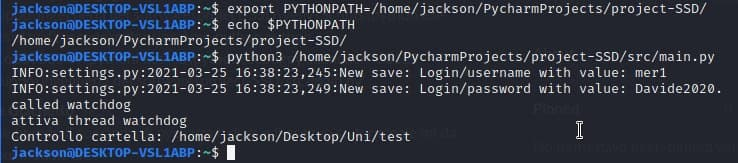
\includegraphics[scale = 0.50]{components/img/linux-istruzione-1.jpg}
    \caption{ Comando per impostare PYTHONPATH su linux}
    \label{fig:comando per impostare PYTHONPATH su windows}
\end{figure}
\subsection{Come avviare il programma}
Con il PYTHONPATH impostato correttamente per avviare il programma si utilizza il comando python3 seguito dal path assoluto del file main.py. Di seguito viene riportato un esempio.
\begin{figure}[H]
    \centering
    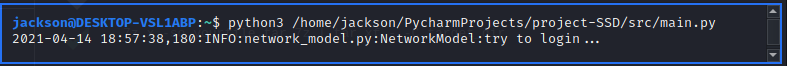
\includegraphics[scale = 0.50]{components/img/avvio.png}
    \caption{ Comando per avviare SSD}
    \label{fig:comando per impostare PYTHONPATH su windows}
\end{figure}